%!TEX root = ../document.tex
\chapter{Evaluation}\label{ch:evaluation}

\begin{quotation}
  {\small\it }"ANOTHER FANTASTIC QUOTE"{\small\it -- FROM SOMEONE FANTASTIC }
\end{quotation}


In this section we evaluate browserCloud.js via real executions on top of increasing number of browsers executing locally, to assess the limits of current Javascript engines on typical desktop machines, and with micro-benchmarks to determine the speedups that can be achieved in distributed executions with one browser per individual desktop machine.

This, in order to assess the potential of the proposed system, we have built a ray-tracing application, adapted from algorithms available, written in full vanilla JavaScript, that can be run on any  typical modern browser engine. This algorithm allows us to stress-test the CPU,  and the possibility to obtain advantages through processing parallelism. We need this to understand whether the expected speeds up resulting from distributing the tasks through the browserCloud.js peers network, are not hindered by loosing efficiency due to message routing on the overlay Network.

When distributing a job through a multiple node network, one of the aspects we observed was that we can influence overall efficiency by adjusting how much resources we are going to take from the network to process the job, in this case, how much browsers. We also can influence it by deciding how much fine-grained each task it will be: the smaller the computation unit, the more we can distribute tasks through the network, with a natural trade-off of adding more task generation and messaging overhead, with diminishing returns when more and more, and  smaller tasks are created.

The standard ray-tracing job using the algorithm developed, running in a single browser takes as median 2361.434s to complete (around 40 minutes). As we can see in Figures~\ref{fig:ray2500}~and~\ref{fig:ray2500time}, our system excels in delivering faster results by dividing the job up to 2500 computational units (or tasks) and requesting from the browsers available in the network to compute those (i.e., a rectangle of the resulting output image). This is expected as ray-tracing is a known case of an embarrassingly parallel application.

One fact interesting to note is that we obtained much better results by reducing the granularity of which ray-tracing job was divided into, as we can see on Figures~\ref{fig:ray25}~and~\ref{fig:ray25time}. This happens due to two factors: a) the first is that since we have a lower number of tasks to be run by other browsers, we reduce the message routing overhead between nodes (i.e., resource discovery does not take so long); b) the second factor is that since this system was tested using a single machine and a networked simulated delay. When the number of tasks is too large, the workers in the browser are in fact competing for CPU resources (to execute tasks and to forward messages among them). This creates a scenario, where more nodes/workers actually  make the system slower, since this is a much more strict and resource constrained scenario, than a real example with browsers executing in different machines.

In a real world example, the actual execution time would be bounded by:\\

$\textbf{jobTime}=slowestDelayFromResourceDiscovery+timeOfExecutingSlowestTask+slowestDelayFromResultReply (1)$ \\

with full parallelism, where in our test scenario we have: \\

$\textbf{jobTime}=\sum{DelayFromResourceDiscovery}+(TimeOfExecuting\_N\_Tasks\_on\_M\_Resources)+\sum{DelayFromResultReply} (2)$\\

where N=2500 and M=8 hardware threads, therefore contention for CPU becomes higher with more nodes (browsers) as more messaging is taking place, besides the parallelized computation.

\begin{figure}[]
  \centering
  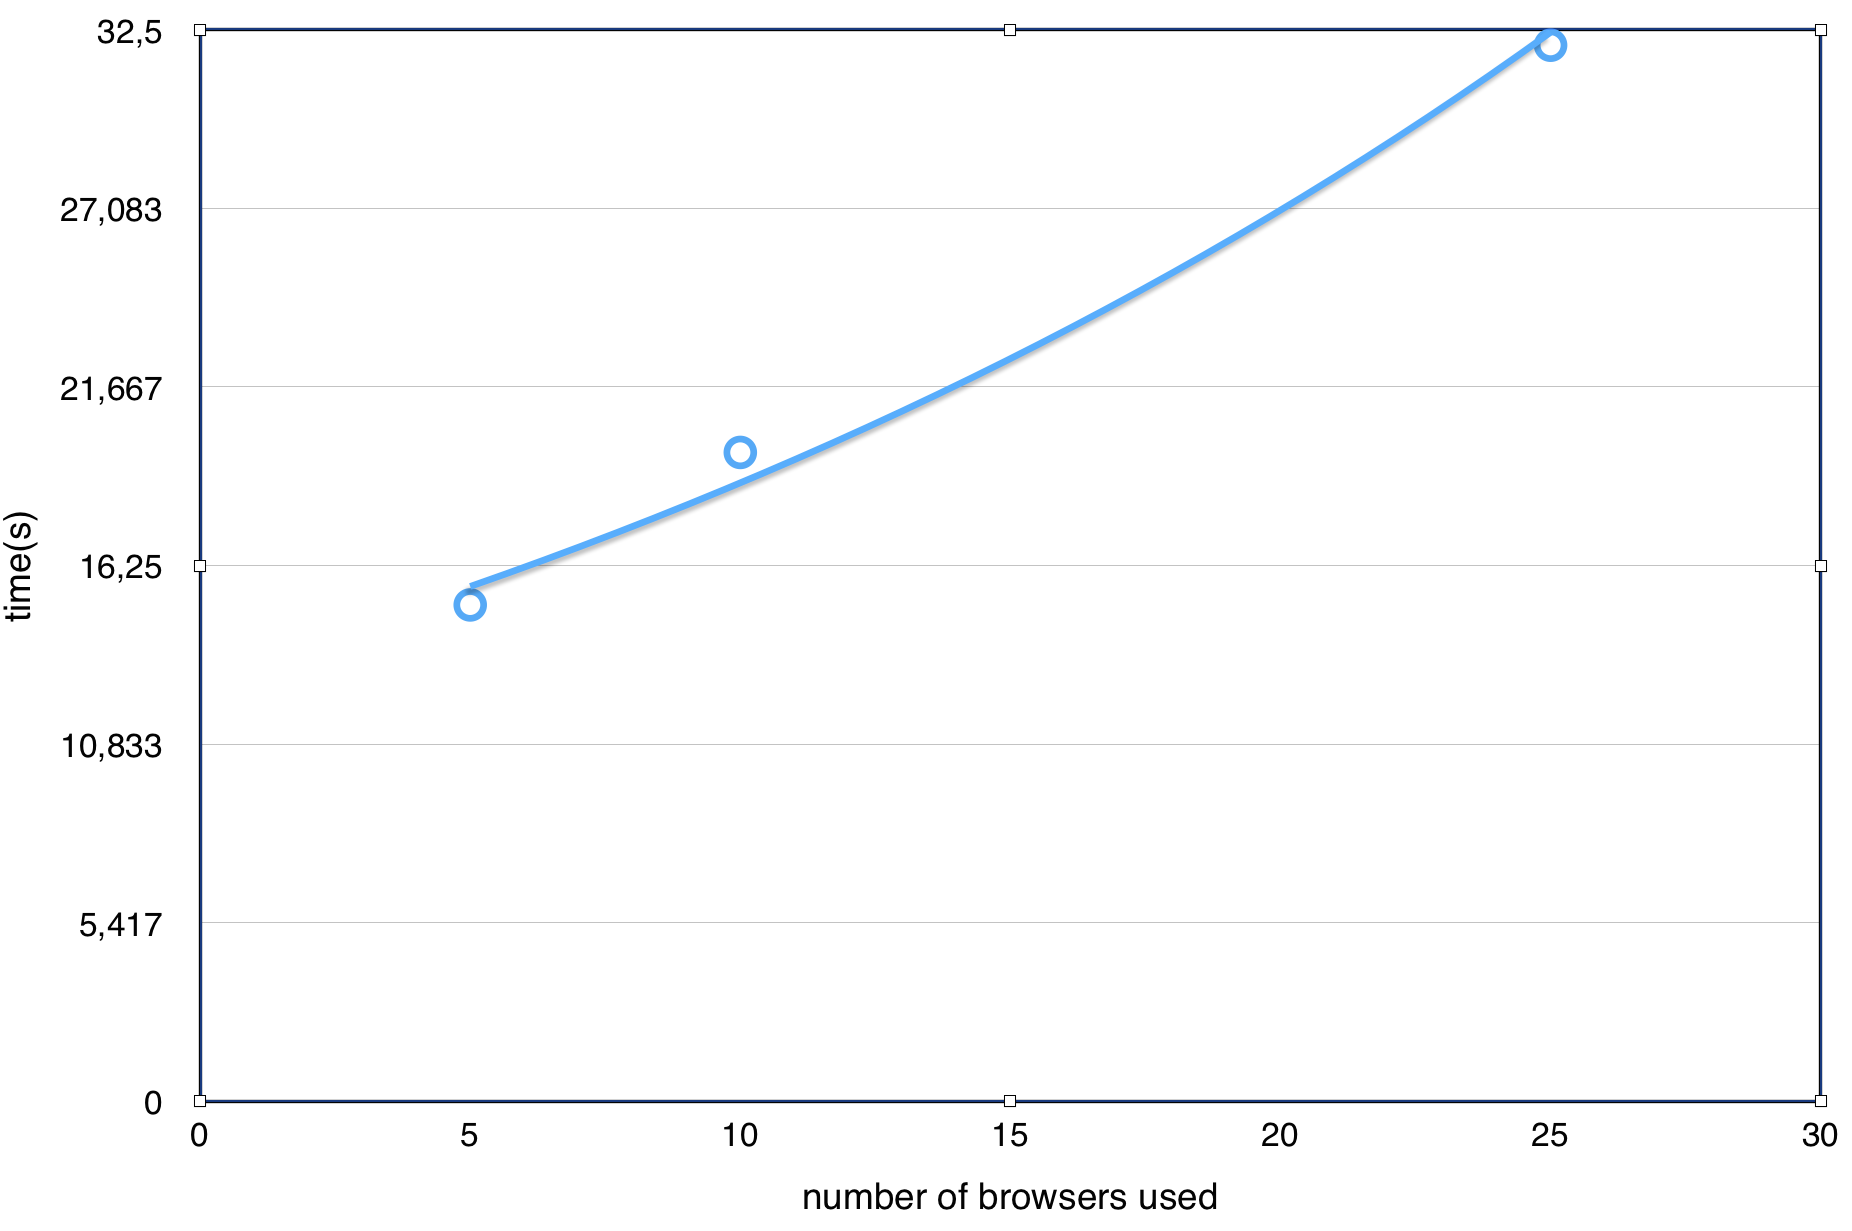
\includegraphics[width=0.5\textwidth]{figs/1.png}
  \caption{Time elapsed on a ray-tracing job divided in 2500 computing units}
  \label{fig:ray2500}
\end{figure}

\begin{figure}[]
  \centering
  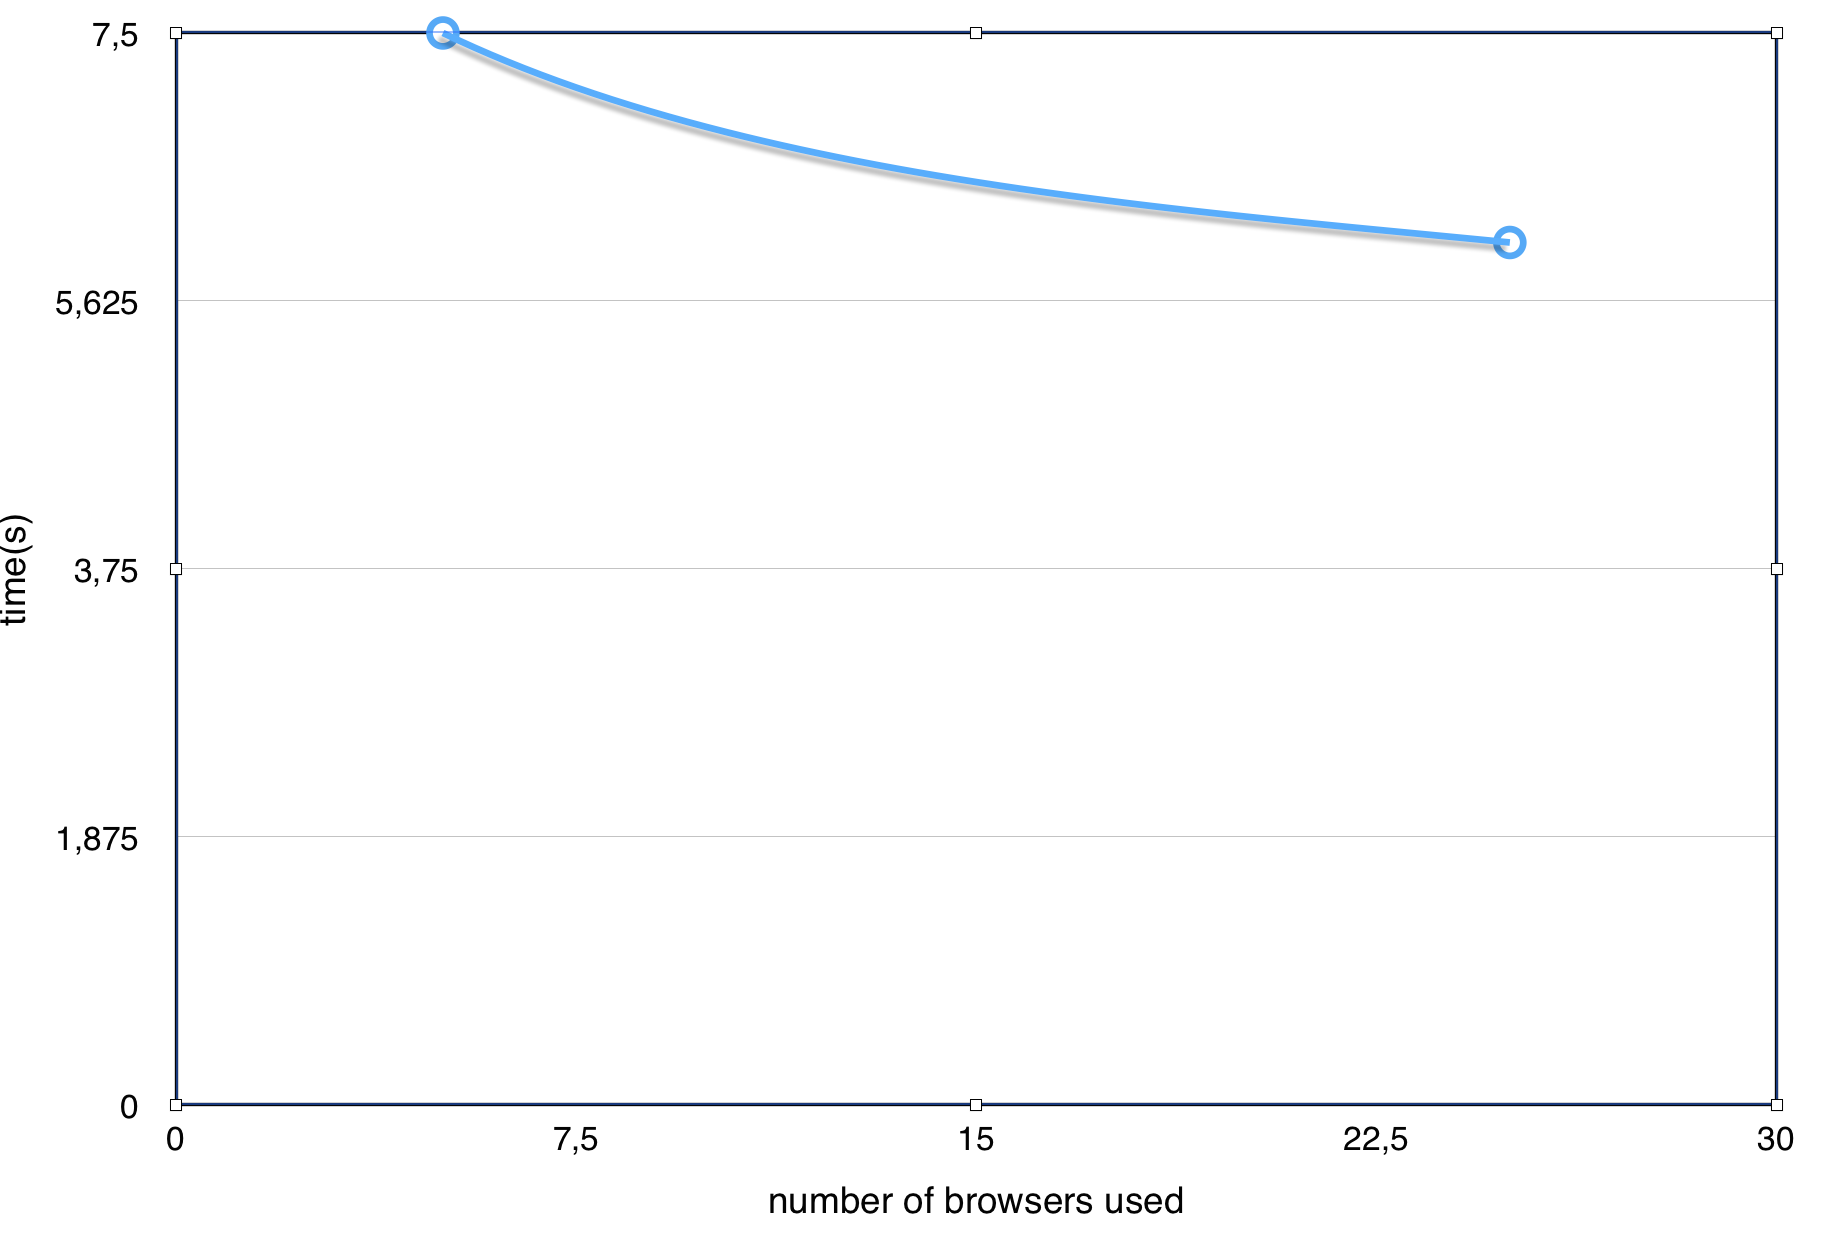
\includegraphics[width=0.5\textwidth]{figs/2.png}
  \caption{Time elapsed on a ray-tracing job divided in 25 computing units}
  \label{fig:ray25}
\end{figure}

\begin{figure}[]
  \centering
  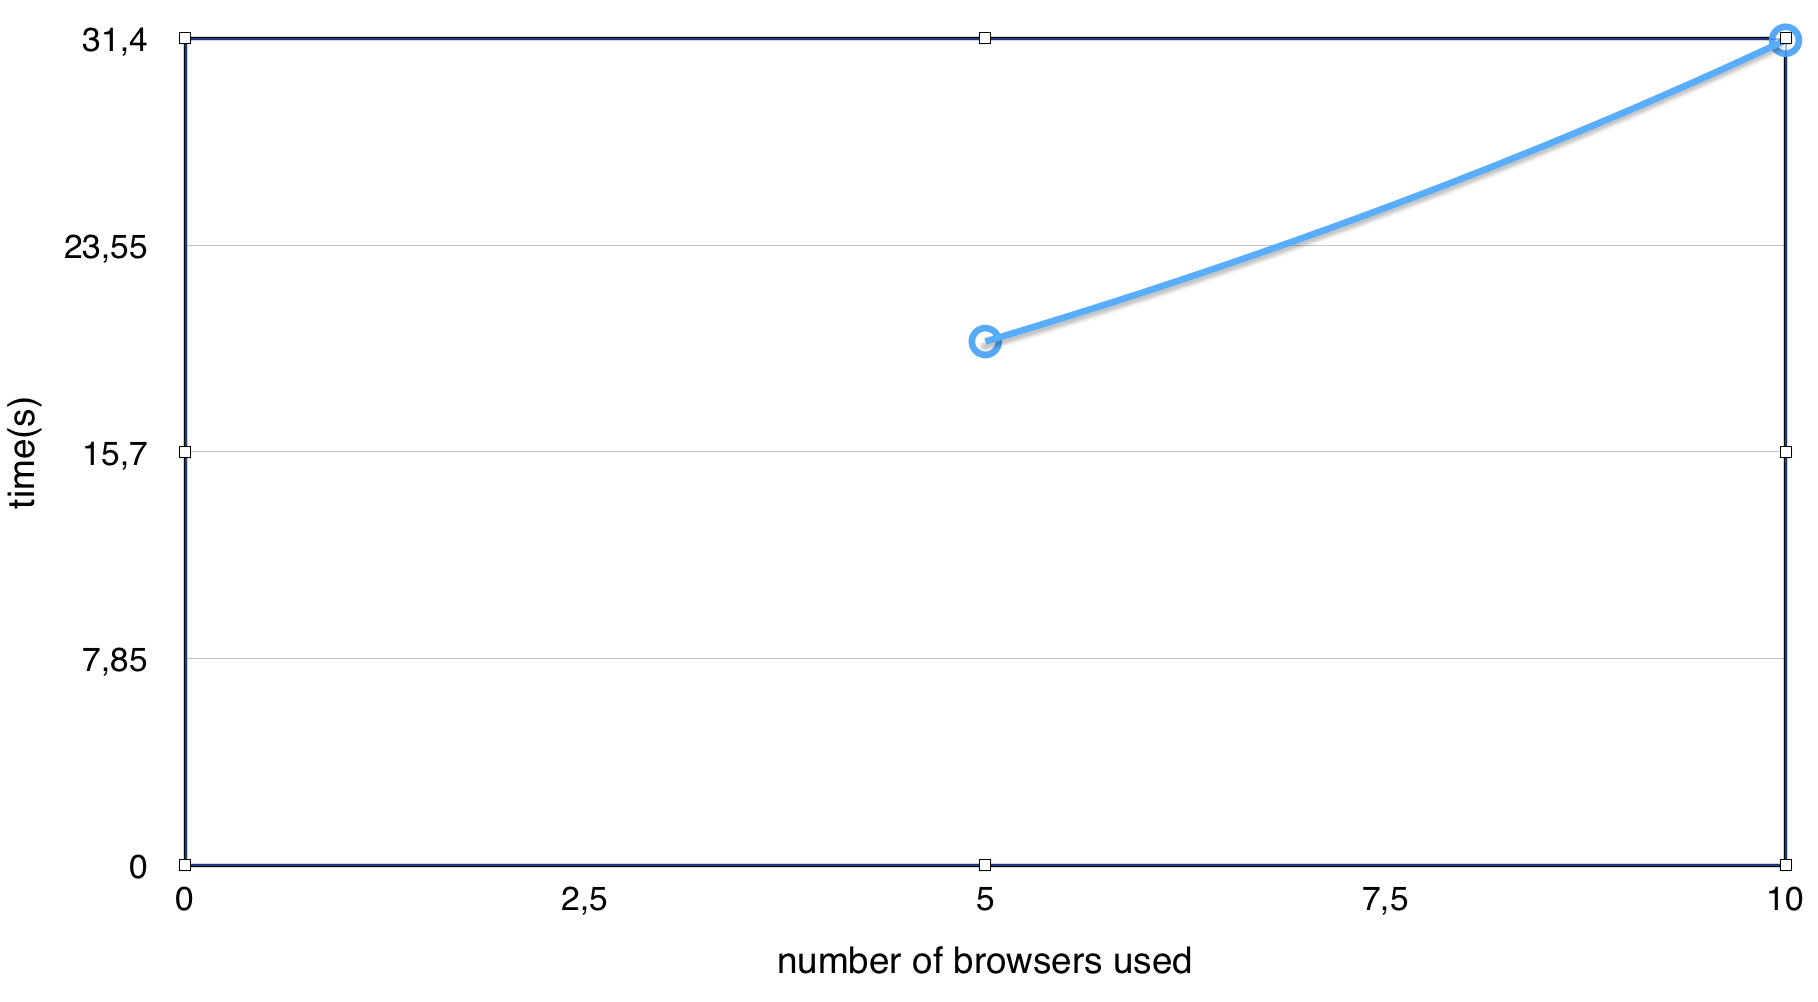
\includegraphics[width=0.5\textwidth]{figs/3.png}
  \caption{Time elapsed on a ray-tracing job divided in 2500 computing units (with induced web RTT delay)}
  \label{fig:ray2500time}
\end{figure}

\begin{figure}[]
  \centering
  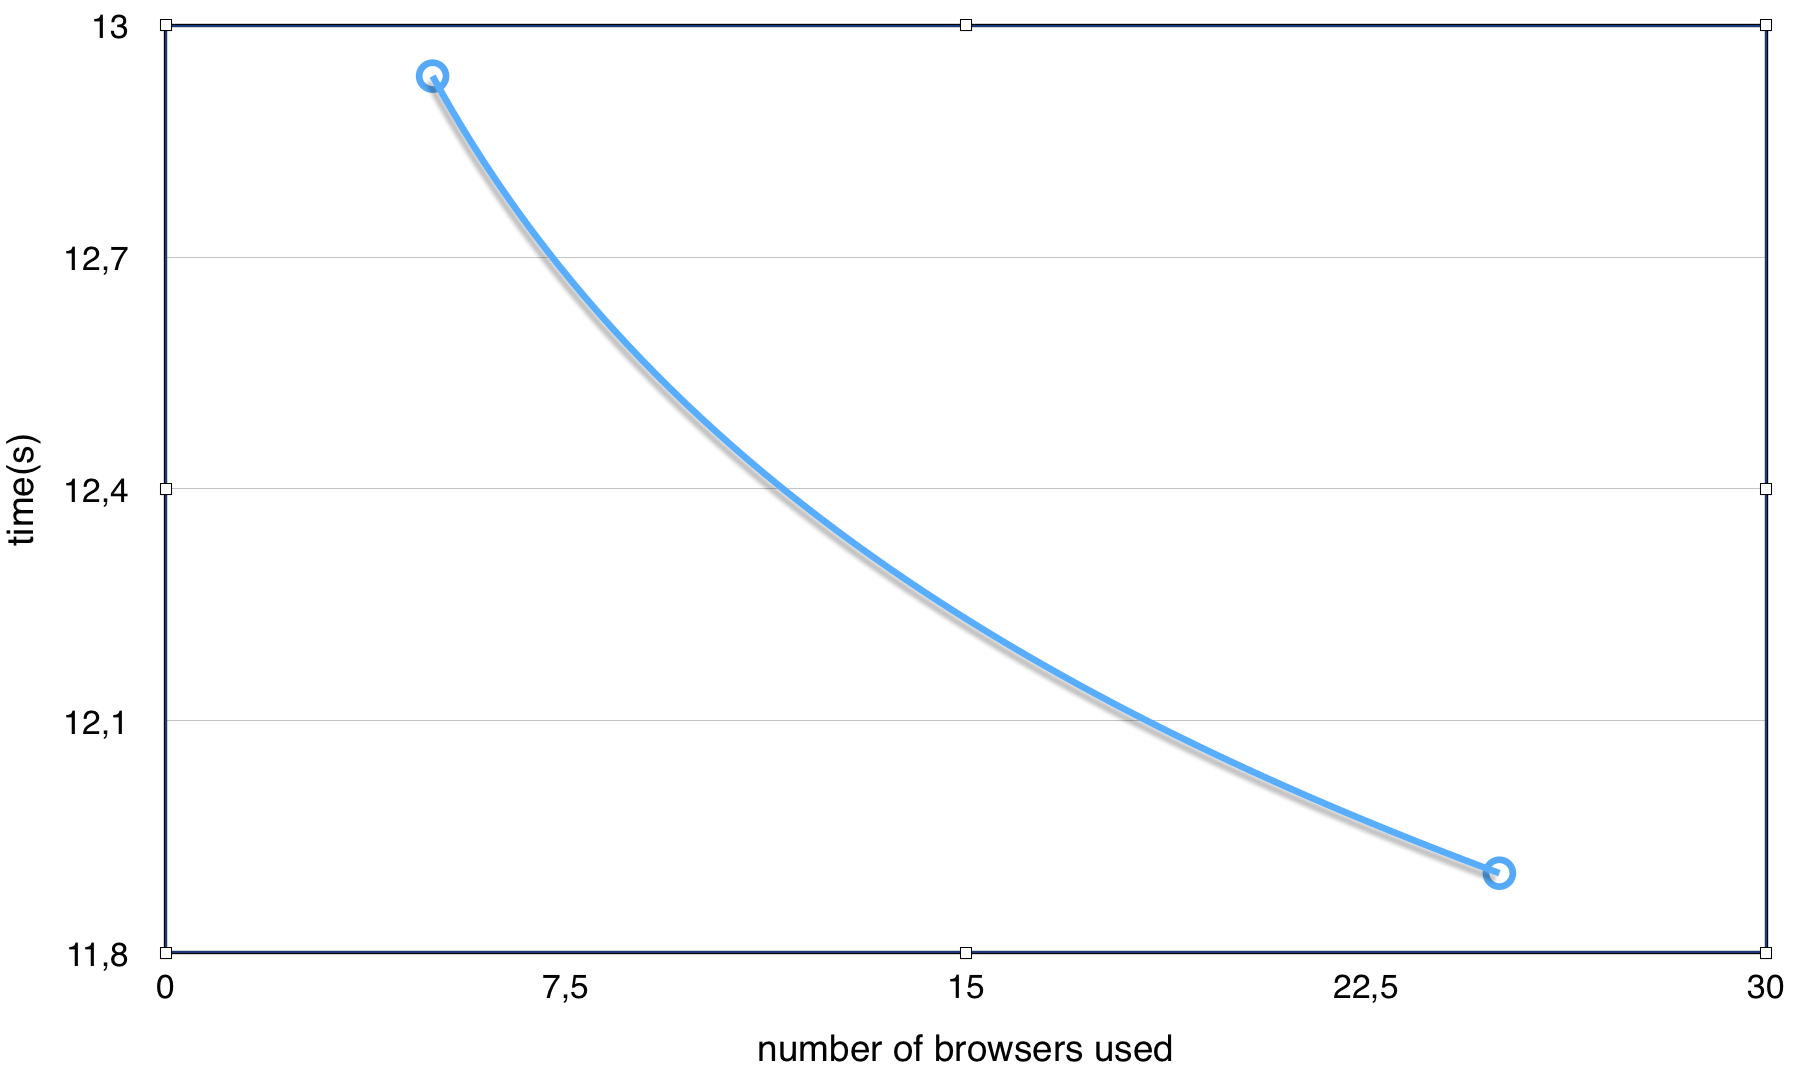
\includegraphics[width=0.5\textwidth]{figs/4.png}
  \caption{Time elapsed on a ray-tracing job divided in 25 computing units (with induced web RTT delay)}
  \label{fig:ray25time}
\end{figure}

In a real world scenario, with more browsers from more machines, the total execution time (makespan) of a ray-tracing job would be closer to that described by Equation 1. It would be influenced by the maximum round trip time between any two nodes (so that the information for every task can be received and processed by another node), plus the time it would take to execute the most of CPU intensive task (e.g., the rectangle in the frame that has the more complex geometry and light reflections to be processed). Figures~\ref{fig:avgtimeexec}~and~\ref{fig:rtt} show what is the average task length and RTT between any two nodes, being the maximum for the first 61ms and the second 11174ms, creating a total of 11235ms (or 11.296s overall). This is a significant increase of efficiency, comparing to the sequential execution (a speedup of about 209 times fold) and also to the previous single-machine experiments.

It is important to note that in Figure~\ref{fig:avgtimeexec}, we can see several task execution lengths due to the complexity of each task, with more or less light reflections. With this microbenchmark we see that the execution time of each task, without any resource contention (1 node = 1 browser per machine), the task duration has an even lower upper bound (lower than 5s). This would entail the upper bound of total task execution time to be under 5061 ms (around just 5s), with a theoretical speedup of about 466 times (take into account that we would be using 2500 nodes then, so speedups are not perfectly linear due to communication overhead, as expected).

\begin{figure}[]
  \centering
  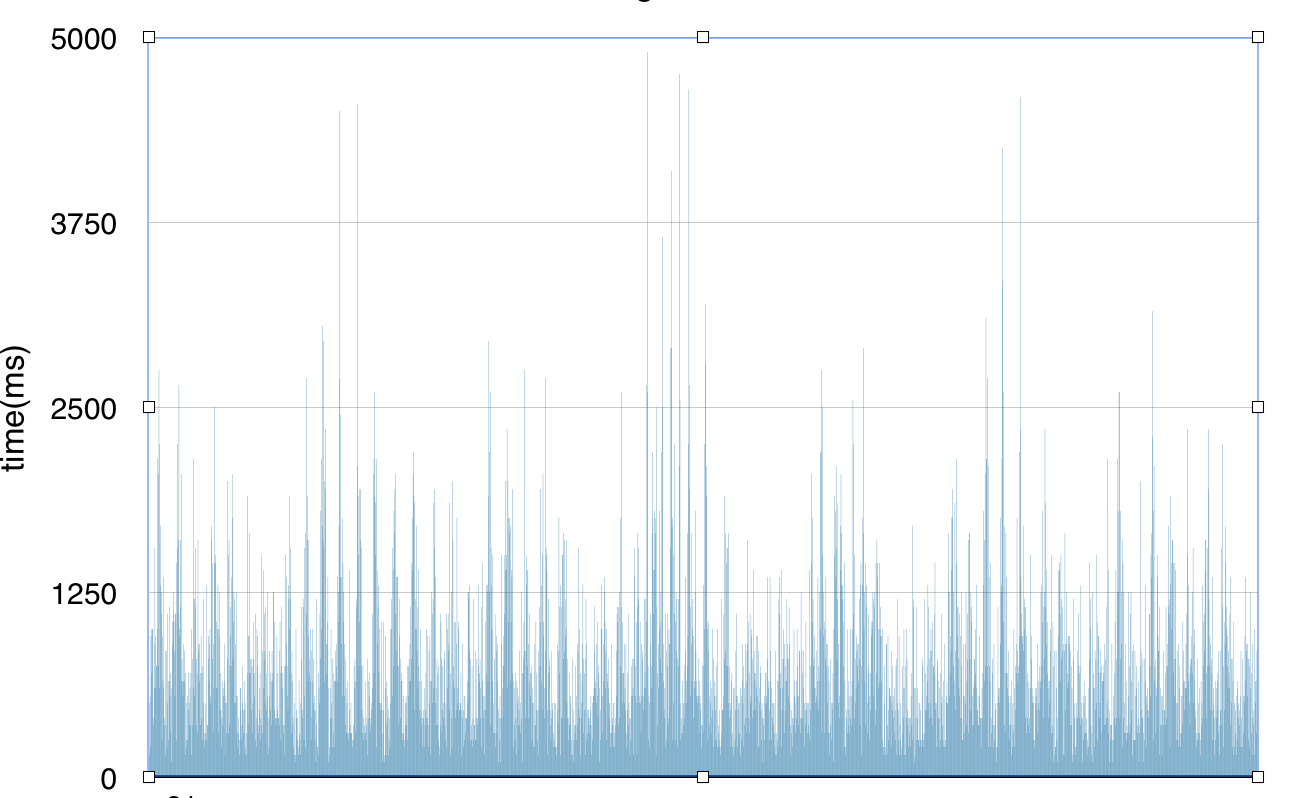
\includegraphics[width=0.5\textwidth]{figs/avg_time_exec.png}
  \caption{Average time for a task execution for a job fragmented in 2500 computing units}
  \label{fig:avgtimeexec}
\end{figure}

\begin{figure}[]
  \centering
  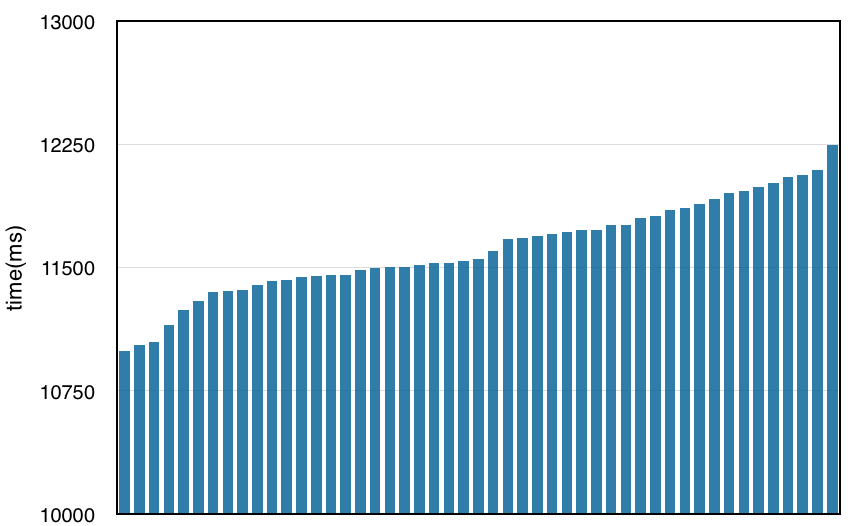
\includegraphics[width=0.5\textwidth]{figs/rtt.png}
  \caption{Average Round Trip Time between an two nodes in a 10 browser network}
  \label{fig:rtt}
\end{figure}


There are also some other performance bottlenecks we noticed that arise from the single threaded nature of JavaScript engines. These aspects are considered in our performance evaluation, such as:

\begin{itemize}
  \item Logging - Since V8 runs in a single thread, any synchronous operation will block the event loop and add delay to the whole processing, although these logs are essential for us to assess the efficiency of the infrastructure, they are not vital to the job.
  \item Delay added - One technique we used to simulate the network delay is to use the `setTimeout' native function of V8's JavaScript implementation, since this function is unable to receive floating millisecond values. Moreover, since `setTimeout' does not necessarily guarantee that the function will be executed in X amount of milliseconds, due to the nature of the event loop, there is always an extra delay added implicitly to the operation in the order of 1 to 3 ms.
  \item Tasks can not be sent in parallel - A node has to send each individual computing unit sequentially and independently, meaning that if we divide a job into 2000 for e.g, each task will have to wait for the previous to be sent.
\end{itemize}

These bottlenecks were studied and will be tackled in future work, one of the solutions proposed is to use Service Workers\cite{ServiceWorkers} for full multithreaded operation inside browserCloud.js.


\section*{Summary}
